\documentclass[a4paper, 12pt]{article}

\usepackage{helvet}
\renewcommand{\familydefault}{\sfdefault}

%\hyphenation
\usepackage{pdfpages}

\usepackage[utf8]{inputenc}  
\usepackage[francais]{babel}
\usepackage[T1]{fontenc}  
\renewcommand{\baselinestretch}{1.5} 

\title{Écrit réflexif : L'évaluation par compétences}
\author{CLIN Exavérine}
\date{2017-2018}

\begin{document}
\maketitle
\thispagestyle{empty}

\newpage
\part*{Remerciements}
% Remerciements

Je remercie la Directrice de l'ESPE d'avoir mis en place ce Master Métiers de l'Enseignement, de l'Education et de la Formation Mention Second Degré Parcours Sciences Industrielles de l'Ingénieur.


%M Inspecteur d'Académie - Inspecteur Pédagogique Régional


Je remercie Monsieur Jolly de m'avoir accueilli au sein de son établissement.


Je tiens à remercier mon tuteur EPLE, Patrick PARENT, pour son soutien tout au long de cette première année d'exercice, ses précieux conseils ainsi que sa disponibilité.

Je remercie également l'ensemble des formateurs ESPE pour les formations qu'ils ont dispensées.




\thispagestyle{empty}
%\addcontentsline{toc}{part}{Remerciements} 

\newpage
\part*{Résumé}
\addcontentsline{toc}{part}{Résumé} 
% Resumé

%\addcontentsline{toc}{part}{Le Monde} 
%\addcontentsline{toc}{chapter}{L'Eurasie} 
%\addcontentsline{toc}{section}{L'Europe} 
%\addcontentsline{toc}{subsection}{La France} 
%\addcontentsline{toc}{subsubsection}{L'Aquitaine} 
%\addcontentsline{toc}{paragraph}{La Gironde} 
%\addcontentsline{toc}{subparagraph}{Bordeaux} 

\newpage
\tableofcontents

\newpage
\part{Introduction}

% Présentation du collège
J'enseigne dans le collège Henry de Montherlant situé à Neuilly-en-Thelle.
Ce collège est un collège sans note, je me suis demandée comment évaluer les élèves moi qui étais habitué aux notes.

% Situation déclanchante
Lors de l'évaluation sommative sur la première séquence j'ai constaté une faible réussite.
J'ai donc remis en cause tout d'abord mon enseignement puis me suis ensuite interrogée sur la façon d'évaluer les élèves.

% Problématique
J'en suis donc arrivé à la problématique suivante : 
Comment évaluer les élèves ?
Quels sont les outils qui permettent une évaluation par compétence?
Comment peut-on rendre les élèves acteurs de leur évaluation ?



\newpage
\part{Situation déclenchante}
% Mise en place de l'évaluation

\section{Évaluation des connaissances}

Ma première séquence était intitulée \og Qu'est-ce qu'un cahier des charges fonctionnel~?\fg. 
Pour cette séquence je n'ai pas réalisé d'évaluation diagnostique afin de déterminer les connaissances des élèves sur le cahier des charges.
Cela fut une première erreur de ma part car je pensais effectuer des rappels avant d'aller plus loin, or pour les élèves les notions de \og diagramme bête à cornes\fg ~et de \og diagramme pieuvre\fg ~n'évoquaient rien.
J'ai donc passé une séance complète sur la réalisation de ces deux diagrammes qui étaient inconnus aux élèves.
Si j'avais effectué une rapide évaluation diagnostique cela m'aurait fait gagner du temps.

Concernant la structure de la séquence sur la réalisation du cahier des charges je demandais énormément d'attention de la part des élèves. 
Effectivement mon cours s'est déroulé de façon magistral avec une partie travaux dirigés durant laquelle les élèves ont réalisés les deux types de diagrammes.
Les élèves n'ont pas communiqués durant les exercices et s'en ai suivie une phase de correction au tableau par des élèves volontaires.

Afin de vérifier que les élèves puissent réaliser par eux même un diagramme bête à cornes je leur ai demandé de réaliser sur une feuille ce diagramme sur différents objets de leur quotidien.

J'ai ensuite poursuivi le cours sur le cahier des charges notamment sur les fonctions principales et fonctions contraintes.

A la fin de la séquence j'ai prévenu les élèves qu'une évaluation aurait lieu la semaine suivante.
Cette évaluation porterait sur la réalisation de deux diagrammes et l'identification de la fonction principale et des fonctions contraintes.
L'évaluation que j'ai réalisé se trouve Annexe~\ref{annexe:evaluation_cdcf}.

\section{Critique}

L'évaluation que j'ai mise en place est une évaluation dite \og classique \fg, elle consiste à évaluer les connaissances des élèves.

Le résultat de cette évaluation, pour la majorité des élèves était mauvais.
Si j'avais obtenu beaucoup de bons résultats je pense que je me serai interrogé sur la qualité de mon évaluation.
Le fait ici d'avoir de mauvaises notes m'a en quelque sort "rassuré" car je n'avais pas sous estimé la capacité des élèves.
De plus lorsqu'un professeur donne de bonnes notes à la classe il peut être considéré comme laxiste ou médiocre.
Une certaine angoisse à avoir des notes trop élevés fait que j'ai noté les élèves sans vraiment me demander si les élèves avaient compris les notions.

Après la lecture de livre d'Antibi sur \og constante macabre \fg je me suis rendu compte qu'il y a de grandes variations de notation suivant les examinateurs, mais aussi d'un même examinateur dans le temps.
De plus l'existance de la \og constante macabre \fg~\cite{antibi2003constante} est aussi un facteur d'influence.
Ce phénomène consiste à attribuer, quelle que soit la qualité des copies, un pourcentage de mauvaises notes.

En lisant ce livre je me suis identifiée aux enseignants qui cherchaient à obtenir une répartition des notes \og 1/3, 1/3, 1/3\fg.
Cette lecture m'a permis de prendre conscience de ce phénomène et de m'interroger sur la façon dont je pouvais évaluer les compétences des élèves en laissant de côté cette constante macabre.

Pour supprimer \og constante macabre \fg, s~\cite{antibi2007notes} propose de mettre en place une évaluation par objectifs.
Cela consiste à déterminer des objectifs clairs et précis que l'élève doit atteindre afin de réussir un contrôle.

Je me suis donc inspiré de cela pour évaluer les compétences des élèves non pas sous la forme d'un contrôle mais avec un objectif à atteindre.

 
\setcounter{section}{0}

\newpage
\part{Définitions de l'évaluation}
\section{L'évaluation}

Au sens étymologique le terme "évaluation" provient de "ex-valuere" qui signifie déterminer la valeur de.

\subsection{Différents types d'évaluation}

Dans la bibliographie il existe de nombreuses définitions de l'évaluation, mais celle de \cite{de_ketele_levaluation_1989} reste parmi les plus complètes.
\og Évaluer signifie
\begin{itemize} 
\item recueillir un ensemble d'informations suffisamment pertinentes, valides et fiables
\item et examiner le degré d'adéquation entre cet ensemble d'informations et un ensemble de critères adéquats aux objectifs fixés au départ ou ajustés en cours de route
\item en vue de prendre une décision \fg
\end{itemize}


Il explique que l'évaluation prépare à une décision mais n'en fait pas partie. 
Le fait de parler de décision est assimilé à un jugement, au fait d'apprécier une personne ou une action. 
Mais l'évaluation, contrairement au jugement, est un processus basé sur des critères explicites.

Pour cela dans son livre, ~\cite{roegiers_lecole_2010} propose trois évaluations des acquis des élèves~:
\begin{itemize}
\item \og en début d'année sur les performances des élèves pour décider si l'on peut commencer les apprentissages comme prévu \fg ~;
\item \og en cours d'année sur les performances d'un élève pour décider s'il est nécessaire de mettre en place une procédure de remédiation \fg ~;
\item \og en fin d'année sur les performances d'un élève pour décider s'il peut passer dans la classe supérieure \fg .
\end{itemize}

Ces trois types d'évaluations se déroule à deux échelles celle de l'élève et celle de la classe.
Concernant l'élève~:
\begin{itemize}
\item L'évaluation qui s'effectue avant l'apprentissage s'appelle l'évaluation d'orientation. Elle permet de diagnostiquer les forces et les faiblesses pour orienter l'élève vers un type d'apprentissage plus adapté. C'est pour cela que l'on parle également d'évaluation diagnostique.
\item L'évaluation qui s'effectue durant l'apprentissage permet de détecter les difficultés au niveau de chaque élève afin d'y remédier. Cette évaluation s'appelle évaluation formative.
\item L'évaluation qui s'effectue en fin d'apprentissage, fin d'année, permet de valider les acquis des élèves, c'est l'évaluation sommative aussi appelée évaluation certificative lorsqu'elle aboutit à la délivrance d'un diplôme ou l'accès à la formation du niveau supérieur.
\end{itemize}

\subsection{Un modèle d'évaluation}

Dans leur livre~\cite{doyon_faire_1991} présente un modèle d'évaluation formative qui fait participer l'élève du primaire à l'évaluation de ses apprentissages. 
Les auteurs proposent un modèle d'auto-évaluation qui a pour objectif d'amener l'élève à devenir de plus en plus autonome.
Ils décrivent un processus d'auto-évaluation cyclique composé de quatre phases qui se déroule à l'intérieur d'une séquence d'apprentissage.
%\begin{enumerate}
%\item Phase de planification~: \og elle consiste à déterminer avec les élèves les objectifs d'apprentissage poursuivis au cours de la séquence, à préciser les critère d'évaluation par des indicateurs d'observation \fg
%\item Phase de réalisation~: \og elle consiste à réaliser les activités d'évaluation prévues, à faire participer l'élève à l'évaluation de ses apprentissages et à consigner les résultats d'évaluation \fg
%\item Phase de communication des résultats~: \og elle consiste à préparer la communication des résultats aux parents, à organiser et à réaliser une rencontre parents-enfants au moment de la remise du bulletin \fg
%\item Phase de prise de décision~: \og  \fg
%\end{enumerate}

Voici la synthèse des quatre phases du processus d'auto-évaluation et les étapes qu'elles renferment~:
\begin{enumerate}
\item Phase de planification
	\begin{itemize}
	\item Détermination des objectifs d'apprentissage poursuivis aux cours de la séquence.
	\item Précision des critères d'évaluation des apprentissages.
	\item Prévision des situations d'apprentissage et d'évaluation.
	\item Préparation des outils de consignation des résultats d'évaluation.
	\end{itemize}
\item Phase de réalisation
	\begin{itemize}
	\item Réalisation des activités d'évaluation.
	\item Autoévaluation de l'élève et consignation de ses observations.
	\item Co-évaluation et consignation des observations de l'enseignant.
	\item Conservation des résultats d'évaluation.
	\end{itemize}
\item Phase de communication des résultats
	\begin{itemize}
	\item Préparation de la communication aux parents.
	\item Organisation de la rencontre parents-enfants.
	\item Réalisation de la rencontre parents-enfants.
	\end{itemize}
\item Phase de prise de décision
	\begin{itemize}
	\item Examen rétrospectif de la rencontre parents-enfants.
	\item Prise de conscience par l'élève de son cheminement et sélection d'objectifs personnels prioritaires.
	\item Sélection d'objectifs collectifs à être poursuivis par la classe.
	\item Vérification des outils de travail de l'élève.
	\end{itemize}
\end{enumerate}

Leur approche étant destinée aux élèves du primaire, je n'ai pas retenu tout le cheminement pour chaque séquence.
Je me suis concentrée sur les deux premières phases, celle de planification et celle de réalisation.


Je me suis inspirée de leur modèle d'évaluation que j'ai adapté au cycle du secondaire.
Retour par les élèves sur leurs apprentissages pour se situer~:
\begin{itemize}
\item J'ai réussi avec facilité et suis allé au-delà de la tâche demandée. 
\item J'ai tout juste réussi à réaliser la tâche demandée.
\item Je n'ai pas réussi à réaliser la tâche demandée, même avec de l'aide.
\end{itemize} 


%%% ----------------- Dans le collège

\section{Mise en place au sein de mon établissement}

Au sein de mon établissement nous utilisons le logiciel Sacoche pour saisir les évaluations et effectuer un suivi des compétences des élèves.
Ce logiciel regroupe les compétences du cycle, lors de la saisie d'une évaluation, l'enseignant choisi les compétences qu'il souhaite évaluer ainsi que le niveau atteint par chacun des élèves.

Les compétences sont évaluées suivant quatre niveaux d'acquisition~:
\begin{itemize}
\item Niveau 1~: Non acquis, ce niveau est identifié dans le collège par deux points rouges. L'élève n'a pas atteint l'objectif.
\item Niveau 2~: En voie d'acquisition, identifié par un point rouge. L'élève a eu quelques difficultés et n'a pas entièrement atteint l'objectif.
\item Niveau 3~: Acquis, identifié par un point vert. L'élève à atteint l'objectif.
\item Niveau 4~: Expert, identifié par deux points verts. L'élève à largement atteint l'objectif qui était fixé.
\end{itemize}

L'évaluation par compétence permet de mettre en évidence les différents savoirs à la différence d'une note globale qui n'identifie pas les points forts et difficultés de l'élève.

%%% -----------------
%%% -----------------

\section{Les compétences}

On identifie quelqu'un de compétent comme ayant des acquis (connaissances, savoir-faire, procédures, etc.) et sachant les mobiliser pour résoudre un problème donné.
En d'autres mots, être compétent c'est vouloir, pouvoir et savoir.

Les savoirs regroupent les connaissances théoriques, la connaissance d'un vocabulaire, des lois et normes.

Le savoir-faire est la maîtrise des modes opératoires et des processus dans une situation spécifique.

Le savoir-être est la façon de se comporter.

Afin de prouver sa compétence, les élèves mobilisent les savoirs, savoir-faire et savoir-être

\setcounter{section}{0}

\newpage
\part{Mise en place d'une évaluation}

%%% ------------------------

\section{Évaluation durant les travaux pratiques}

Durant la séquence 2 intitulée \og Comment aménager un lotissement~? \fg \ j'ai commencé par présenter les compétences travaillées par les élèves durant la première séance.
Puis j'ai expliqué l'activité sur laquelle ils seront évalués~: afin de faire venir de nouveaux habitants dans sa commune, le maire de Neuilly-en-Thelle souhaite créer un nouveau lotissement pour accueillir des terrains à bâtir.
L'objectif est d'installer un maximum de terrains à bâtir dans l'espace disponible mais afin de garantir le confort des nouveaux habitants, le constructeur préconise des dimensions à respecter.
Bien entendu chaque terrain à bâtir doit être relié à la route.

Pour cela les élèves sont répartis par groupe de 4 et ont à leur disposition un plan du lotissement à l'échelle $1:50$, des rectangles, chacun représentant un terrain à bâtir avec les dimensions imposées ainsi que des feuilles dans lesquelles ils devront découper les routes, la largeur des routes est aussi imposée.

Les élèves travaillent sur le cahier des charges ainsi que la représentation d'une solution technique à un problème posé.
Ils sont évalués sur leur réalisation, c'est-à-dire le respect du cahier des charges ainsi que l'optimisation de l'espace occupé.

Durant l'activité les élèves étaient investis dans leur travail, ils ont testé plusieurs répartitions spatiales afin de trouver la plus optimisée.
Les compétences que les élèves ont travaillées sont majoritairement acquises excepté un groupe qui n'a positionné aucune route pour relier les terrains à bâtir au reste de la commune.


%%% ------------------------

\section{Donner les clés de la réussite aux élèves}

Lors du lancement de la séquence 4 intitulée \og Comment évoluent les objets techniques~?\fg j'ai présenté les compétences travaillées mais j'ai aussi fourni aux élèves une fiche qui détaille les objectifs à atteindre pour les différents niveaux d'acquisition. 
Chaque compétence est découpée en trois objectifs décrit sur la feuille distribuée, chaque objectif validé rapporte 1 point. Suivant le nombre de point sur chaque compétence l'élève obtient soit Insuffisant (0 point), Fragile (1 points), Acquis (2 points), Expert (3 Points).

L'objectif de l'activité évaluée était de réaliser, par binôme, une frise chronologique sur l'évolution d'un objet technique de leur choix avec le logiciel \textit{OpenOffice Dessin}.

Lors de l'activité les élèves étaient impliqués dans leur évaluation, ils ont régulièrement regarder la fiche d'évaluation pour se positionner.


\section{Permettre aux élèves de choisir leur évaluation}

A la fin de la séquence 5 intitulée \og Comment fonctionnent les objets techniques~?\fg j'ai mis en place une évaluation différenciée.

Durant cette séquence les élèves ont étudiés la chaîne d'énergie de différents objets techniques ainsi que les blocs fonctionnels qui la compose.

Afin de vérifier l'acquisition de la compétence j'ai programmé une évaluation sur feuille.
Étant donné que durant les travaux dirigés certains élèves étaient en difficulté j'ai décider de mettre en place une évaluation différenciée, c'est-à-dire que j'ai proposé aux élèves deux sujets.

Le premier sujet parcours toutes les connaissances vues en classe et demande tout d'abord de représenter le schéma de la chaîne d'énergie sans aucune indication puis de réaliser la chaîne d'énergie de différents objets techniques.
Ce sujet (voir Annexe~\ref{annexe:evaluation_chaine_energie_A}) évalue la compétence sur tout le niveau d'acquisition (Insuffisant, Fragile, Acquis, Expert).

Le second (voir Annexe~\ref{annexe:evaluation_chaine_energie_B}) sujet s'adresse aux élèves ayant eu des difficulté durant les travaux dirigés.
Il évalue la compétence sur les trois premiers niveaux d'acquisition, cela signifie que les élèves qui ont choisi ce sujet ne pourront pas valider la compétence avec le niveau expert.
En effet, ce sujet demande de compléter le schéma de la chaîne d'énergie qui est représenté puis de réaliser ce schéma avec plusieurs objets techniques qui ont étés vu en cours.

J'ai constaté que certains élèves ne savent pas se positionner sur leur connaissances et compétences et donc hésite sur le sujet qu'ils souhaitent traiter.


%%% ------------------------

\section{Permettre à chacun de se situer }

La séquence 7 est intitulée \og Comment fonctionne une écluse~? \fg{}.
Cette séquence se déroule en deux parties~:
\begin{itemize}
\item Découverte des éléments de l'ouvrage d'art puis du fonctionnement de celui-ci en utilisant une application flash. Les élèves devront réaliser une présentation en utilisant \textit{OpenOffice Présentation} dans laquelle ils détailleront les étapes pour permettre à l'écluse de laisser passer un bateau.
\item Étude des étapes de fonctionnement, après une explication sur la réalisation d'un organigramme, les élèves devront réaliser l'organigramme de l'écluse puis de divers objets techniques.
\end{itemize} 

Durant la présentation de la première partie sur le fonctionnement d'une l'écluse, j'ai expliqué aux élèves qu'ils seront évalués sur la réalisation d'une présentation sur le fonctionnement d'une l'écluse.
Pour cela, je leur ai présenté puis distribué la fiche d'évaluation sur laquelle je détaille les objectifs à atteindre pour valider la compétence (voir Annexe~\ref{annexe:evaluation_fct_ecluse}).
En plus de cette évaluation, je demande un retour des élèves sur leur ressentit durant l'activité.

La seconde activité porte sur la réalisation d'organigrammes.
Les élèves ont tout d'abord complété des organigrammes à trous puis ils ont réaliser les organigrammes uniquement à l'aide d'un texte qui décrit le fonctionnement de l'objet technique.

Afin d'aider les élèves à se positionner, j'ai donc choisi d'utiliser les outils numérique et notamment le logiciel Tactileo. 
Ce logiciel m'a permis de créer un contenu multimédia interactif.
Les élèves s'enregistrent avec leur nom et prénom puis visualisent et répondent aux questions du contenu.
Il peut être utilisé via un ordinateur, une tablette ou un smartphone.
Pour cette séquence j'ai personnaliser un parcours, c'est-à-dire que, si un élève n'a pas répondu correctement à une question, je le réoriente vers une ressource numérique pour qu'il revoit la notion puis vers une question similaire. Cet outil permet de faire une personnalisation et différentiation en créant des parcours complets.

La réalisation de ce parcours par les élèves leur à permis de pouvoir se positionner pour le choix d'un des deux sujets d'évaluation.


\section{Associer les compétences aux questions et objectifs}

Je n'ai pas eu l'occasion de pouvoir poursuivre davantage ma réflexion sur l'évaluation des compétences mais j'ai réfléchi à quelques améliorations que je peux apporter.

Pour la séquence suivante je penses intégrer directement l'évaluation dans le sujet de travaux pratiques que je proposerai aux élèves.
Au fur et à mesure de la lecture du sujet, pour chaque objectif les élèves verront directement les sous-objectifs à atteindre pour valider le niveau de compétence associé.

Concernant les sujets d'évaluation sur feuille, je préciserai pour chaque question la compétence évaluée.
Je proposerai également de donner comme devoir à la maison, après les résultats d'évaluation, les sujets plus compliqués aux élèves ayant fait le sujet plus faibles et ayant bien réussi.
Cela permettra à ces élèves de se rendre compte de la différence de difficulté avec leur sujet qu'ils ont choisi et peut-être les inciter à la prochaine évaluation de choisir le sujet permettant de valider la maitrise experte de la compétence.

De plus la réflexion de \cite{antibi2007notes} concernant le système d'évaluation par contrat de confiance me semble intéressant et j'envisage de le mettre en place pour les séquences suivantes.

%%% ------------------------



\setcounter{section}{0}

%\newpage
%\part{??}
%\input{parties/4-eleves}

\newpage
\part{Conclusion}









\newpage
\part*{Bibliographie}
\addcontentsline{toc}{part}{Bibliographie} 
\bibliographystyle{apalike}%plain}
\bibliography{evaluation_competence}


\newpage
\part*{Annexes}
\addcontentsline{toc}{part}{Annexes} 
% Annexe 1 : CDCF
\section{Evaluation cahier des charges fonctionnel}\label{annexe:evaluation_cdcf}
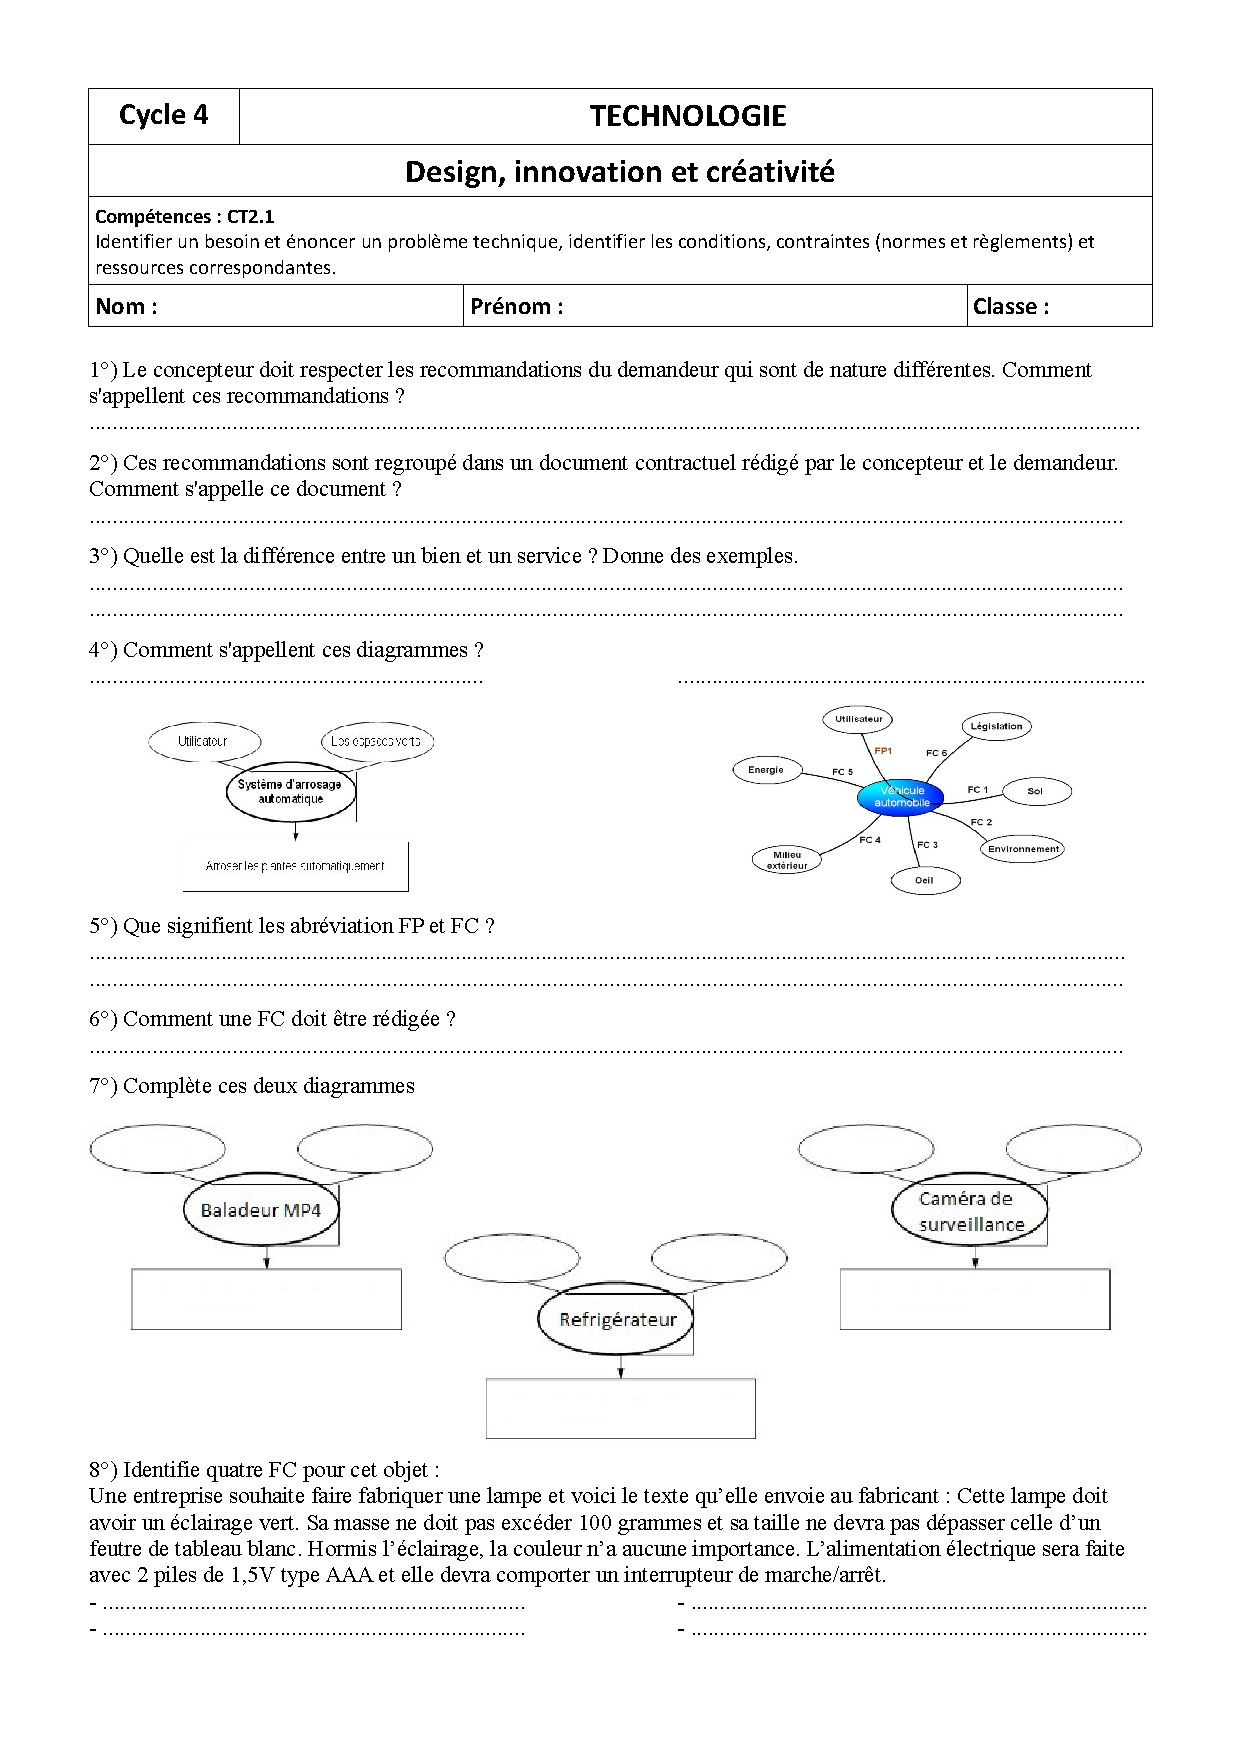
\includegraphics[scale=0.7]{./ressources/Controle_CDCF.pdf} 

\section{Fiche évaluation sur la réalisation d'une frise chronologique}\label{annexe:evaluation_frise}
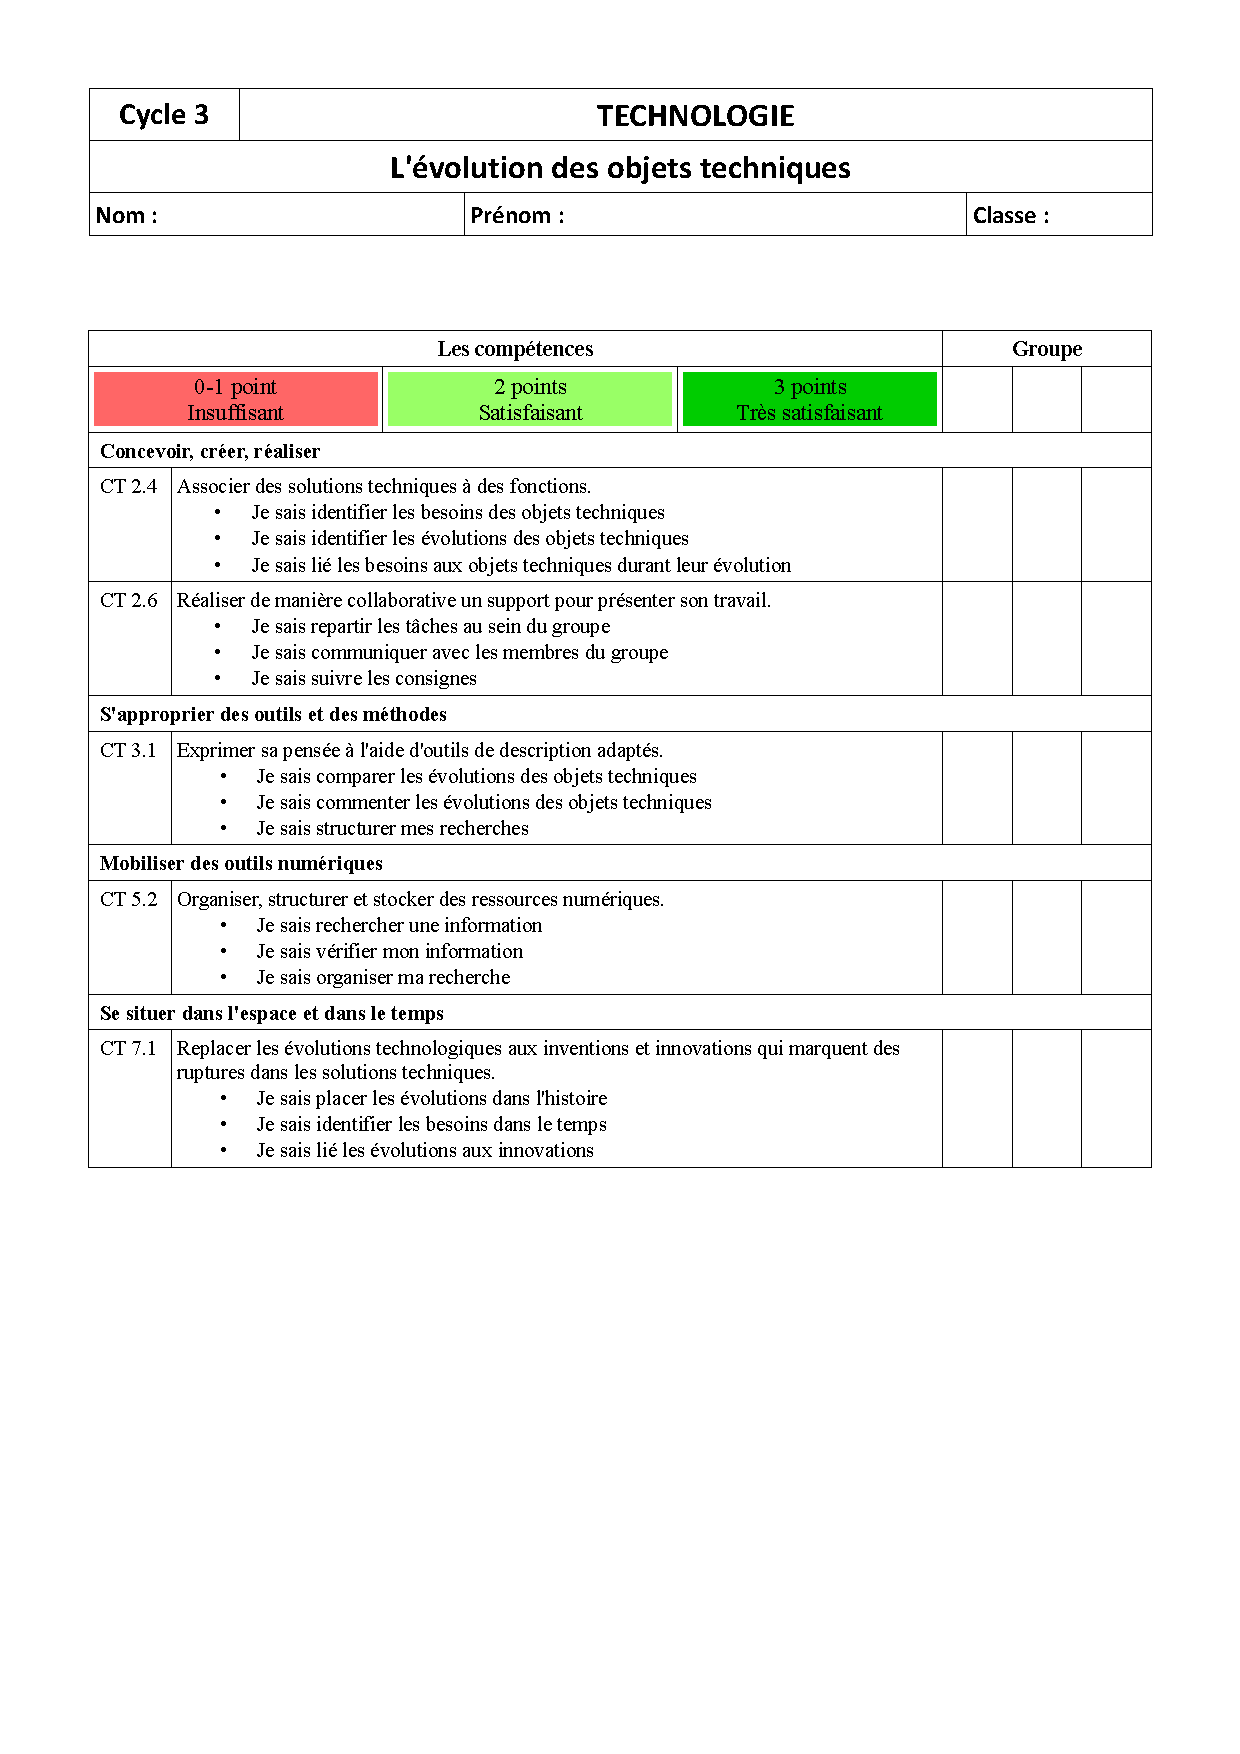
\includegraphics[scale=0.7]{./ressources/TP_evolution_objet_technique_4e.pdf} 

\section{Evaluation différenciée sujet A}\label{annexe:evaluation_chaine_energie_A}
\includegraphics[scale=0.7]{./ressources/Controle_chaine_energie_A.pdf} 

\section{Evaluation différenciée sujet B}\label{annexe:evaluation_chaine_energie_B}
\includegraphics[scale=0.7]{./ressources/Controle_chaine_energie_B.pdf} 

\section{Fiche évaluation sur le fonctionnement de l'écluse}\label{annexe:evaluation_fct_ecluse}
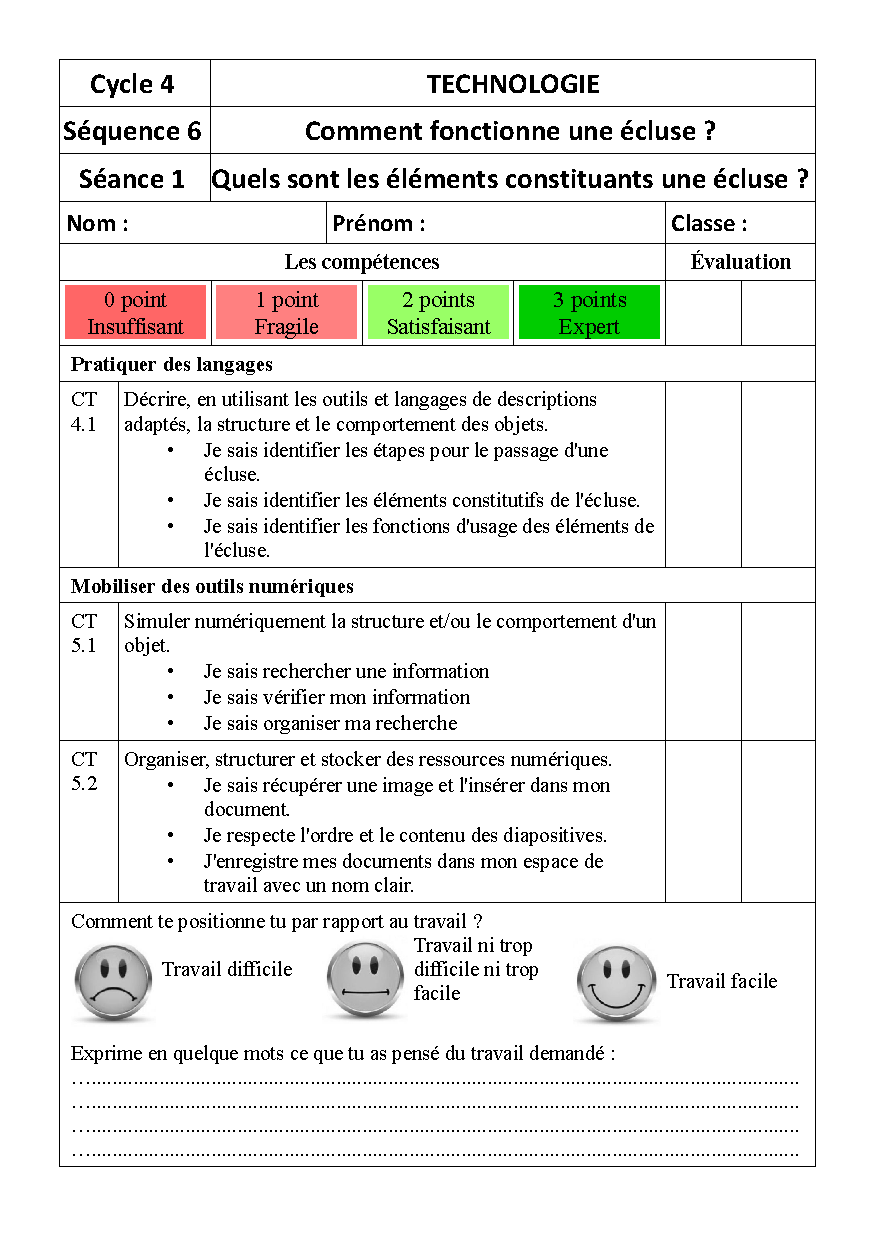
\includegraphics{./ressources/Fonctionnement_Ecluse_S1_4e_a5_1.pdf} 

%\section{Evaluation cahier des charges fonctionnel}\label{annexe:evaluation_cdcf}

% Fiche séquence evaluation

\end{document}
